
%%%%%%%%%%%%%%%%%%%%%%%%%%%%%%%%%%%%%%%%%%%%%%%%%%%%%%%%%%%%%%%%%%%%%%%%%%%%%%%%
\chapter{Implementation}
\label{sct:implementation}
%%%%%%%%%%%%%%%%%%%%%%%%%%%%%%%%%%%%%%%%%%%%%%%%%%%%%%%%%%%%%%%%%%%%%%%%%%%%%%%%


%%%%%%%%%%%%%%%%%%%%%%%%%%%%%%%%%%%%%%%%%%%%%%%%%%%%%%%%%%%%%%%%%%%%%%%%%%%%%%%%
\section{Monte-Carlo-Algorithmen}
\label{sct:montecarloalgo}
%%%%%%%%%%%%%%%%%%%%%%%%%%%%%%%%%%%%%%%%%%%%%%%%%%%%%%%%%%%%%%%%%%%%%%%%%%%%%%%%

Monte-Carlo-Algorithmen sind Algorithmen, die mit Hilfe von (Pseudo-)Zufallszahlen das gesuchte Ergebnis statistisch approximieren. Dafür werden Stichproben aus statistischen Verteilungen durch z.B. physikalisch begründete Abbildungen transformiert und jene Ergebnisse statistisch ausgewertet. Diese Art von Verfahren eignet sich z.B. zur Berechnung von sehr hochdimensionalen Integralen, die mit üblichen Newton-Cotes-Formeln nicht praktikabel wären. Eine andere Anwendung ist die Analyse von durch kosmischer Strahlung ausgelösten Teilchenschauern mit Hilfe von Markov-Ketten\cite{metropolis1949monte}.

Monte-Carlo-Algorithmen sind als statistische Stichprobenverfahren schon länger bekannt, wurden aber erst mit dem Aufkommen der ersten Computer, z.B. dem ENIAC um 1947-1949, praktikabel\cite{metropolis1987beginning}. Der Name, nach der Spielbank ''Monte-Carlo'', wurde von N.Metropolis vorgeschlagen und hielt sich seitdem. Der Vorschlag zu dieser Art von Algorithmus kam von John von Neumann, als man mit dem ENIAC thermonukleare Reaktionen simulieren wollte. Aber Fermi wird nachgesagt schon Jahre zuvor statistische Stichprobenverfahren in schlaflosen Nächten händisch angewandt zu haben und mit den überraschend genauen Resultaten seine Kollegen in Staunen versetzt zu haben.

Monte-Carlo-Verfahren sind inhärent leicht zu parallelisieren, da eine Operation, z.B. die Simulation, mehrere Tausend oder Milliarden Mal ausgeführt wird, jeweils mit unabhängigen Zufallseingaben. Eine Schwierigkeit besteht jedoch darin den Pseudozufallszahlengenerator (pseudorandom number generator - PRNG) korrekt zu parallelisieren. Das heißt vor allem muss man unabhängige Startwerte finden und an die parallelen Prozesse verteilen.

%%%%%%%%%%%%%%%%%%%%%%%%%%%%%%%%%%%%%%%%%%%%%%%%%%%%%%%%%%%%%%%%%%%%%%%%%%%%%%%%
\section{Berechnung von Pi}
%%%%%%%%%%%%%%%%%%%%%%%%%%%%%%%%%%%%%%%%%%%%%%%%%%%%%%%%%%%%%%%%%%%%%%%%%%%%%%%%

Um Pi zu berechnen wird Pi als Integral über eine Kreisfläche dargestellt. Dieses beschränkte Integrale lässt sich nun durch Monte-Carlo-Verfahren approximieren.
\begin{equation}
    \pi = \int_\mathbb{R} \mathrm{d}x
          \int_\mathbb{R} \mathrm{d}y
          \underbrace{\begin{cases}
              1 & |x^2+y^2| \leq 1\\
              0 & \text{sonst}
          \end{cases}}_{=:f(x,y)}
\end{equation}

Da es programmatisch einfacher ist Zufallszahlen aus dem Intervall $[0,1]$ anstatt $[-1,1]$ zu ziehen, wird das Integral über den Einheitskreis in ein Integral über einen Viertelkreis geändert:
\begin{equation}
    \label{eq:piint}
    \pi = 4 \int\limits_{0}^\infty \mathrm{d}x
            \int\limits_{0}^\infty \mathrm{d}y
            \begin{cases}1 & |x^2+y^2| \leq 1\\0 & \text{sonst} \end{cases}
\end{equation}

%Das Vorgehen ist nun wie folgt
%\begin{enumerate}
%    \item Setze die Zählvariable \texttt{Summe} auf $0$
%    \item Ziehe für $x$ und $y$ je eine gleichverteilte Zufallszahl aus dem Intervall $[0,1]$\
%    \item Falls $x^2+y^2<1$, dann erhöhe \texttt{Summe} um $1$
%    \item Gehe zu 2.
%\end{enumerate}

Das Integral aus \autoref{eq:piint} wird nun approximiert:
\begin{equation}
    \label{eq:pimonteint}
    \mu_N = \langle f\left( \vec{x}_i \right) \rangle
          := \frac{1}{N} \sum_{i=1}^N f\left( \vec{x}_i \right),\;
          \vec{x}_i \text{ uniform zufallsverteilt aus } \Omega:=[0,1]\times[0,1]
\end{equation}
Im Allgemeinen ist $f$ eine beliebige Funktion, aber für die Berechnung von Pi ist $f$ die Einheitskugel in 2D, vgl. \autoref{eq:piint}. Gemäß dem Gesetz der großen Zahlen ist dann $\lim\limits_{N\rightarrow \infty} \mu_N = \pi$. Für den algorithmischen Ablauf siehe Algortihmus~\ref{alg:montepi}

\begin{algorithm}
    \DontPrintSemicolon
    \SetKwData{sum}{sum}
    \SetKwData{x}{x}
    \SetKwData{y}{y}
    \SetKwFunction{UniformRandom}{UniformRandom}
    \SetKwInOut{Input}{Eingabe}
    \SetKwInOut{Output}{Ausgabe}
    \Input{Anzahl an Zufallsziehungen $N$}
    \Output{Approximation von $\pi$}
    \BlankLine
    \sum$\leftarrow 0$\;
    \For{ $i\leftarrow 1$ \KwTo $N$ }{
        \x$\leftarrow$\UniformRandom{0,1}\;
        \y$\leftarrow$\UniformRandom{0,1}\;
        \If{$x^2+y^2<1$}{
            \sum$\leftarrow$\sum$+1$\;
        }
    }
    \caption{Berechnung von Trägern mittels Stichproben}
    \label{alg:montepi}
\end{algorithm}

%In Python kann man dies, wenn man sich auf Einkernprozessoren einschränkt, mit NumPy\cite{numpy} in nur wenigen zeilen niederschreiben:
%\begin{lstlisting}[language=python]
%from numpy import *
%N=10000000
%x=random.rand(N)
%y=random.rand(N)
%pi = 4.0 * sum( x*x + y*y < 1 ) / N
%\end{lstlisting}\vspace{-1.5\baselineskip}

Der Vollständigkeit halber seien kurz ein paar Worte zu den Rändern erwähnt; das betrifft die Zufallszahlen die entweder aus einem rechtsoffenem oder abgeschlossenen Intervall $[0,1]$ stammen können, d.h. der Vergleich schließt die Gleichheit mit ein oder nicht.

Aus der Integraltheorie ist klar, dass die Ränder ein Nullmaß haben und damit keine Rolle spielen. Aber für diskrete Verfahren könnte dies zu einer zusätzlichen systematischen Fehlerquelle führen, die das Fehlerskalierverhalten möglicherweise beeinträchtigt.

Am Beispiel von nur vier Zuständen für Zufallszahlen für den rechtsoffenen Fall, also $x,y\in \lbrace 0,0.25,0.5,0.75 \rbrace$, sei dies einmal durchdacht. Damit ergibt sich
\begin{equation}
    x^2+y^2 = \lbrace 0, 0.0625, 0.125, 0.25, 0.3125, 0.5, 0.5625, 0.625, 0.8125, 1.125 \rbrace
\end{equation}
% (Python-Skript für Kombinationen:
%    x=array([0,1,2,3])/4.
%    a,b=meshgrid(x**2,x**2)
%    unique( (a+b).ravel() )
Hier macht es aufgrund der begrenzten Anzahl an Zuständen, unter denen die $1.0$ ohnehin nicht auftritt, keinen Unterschied ob man $<$ oder $\leq$ vergleicht, man erhielte Pi zu $3.6$.
Hinzu kommt aber, dass Zustände auf den Grenzen $x=0$ und $y=0$ liegen, sodass die Grenzen vierfach gezählt werden, wenn die Resultate des Viertelkreis mit vier multipliziert werden.

Man hat also ohnehin immer einen Diskretisierungsfehler von $\mathcal{O}\left(\Delta x\right)$ wobei $\Delta x$ die Diskretisierungslänge zwischen zwei Zuständen ist. Angemerkt sei, dass sich dies für Gleitkommazahlen komplizierter gestaltet.

Abschließend sei angemerkt, dass Monte-Carlo-Methoden dafür gedacht sind einen praktisch unerschöpflichen Raum stichprobenartig auszutesten, sodass Diskretisierungs- und Randfehler ohnehin als vernachlässigbar angenommen werden.
Wenn man merkt, dass es zu Diskretisierungsfehler wie obig an den Rändern kommt, oder man gar die Anzahl aller möglichen Zustände an Zufallszahlen erschöpft hat und sich die Approximation damit nicht mehr verbessern kann, sollte man über ein anderes Verfahren nachdenken oder den Zufallsgenerator anpassen und z.B. mit 128-Bit statt 32-Bit betreiben.
Auch die maximale Periodenlänge von Pseudozufallsgeneratoren spielt hier eine Rolle!

Da die Monte-Carlo-Pi-Integration einer Mittelwertbildung entspricht, vgl. Gl.\ref{eq:pimonteint}, ist die statistische Unsicherheit durch die Standardabweichung des Mittelwerts $\sigma_{\mu_N}$ gegeben.
\begin{equation}
    \sigma_{\mu_N} = \frac{\sigma}{\sqrt{N}}
\end{equation}
wobei $\sigma$ die Standardabweichung der Stichprobe ist, vgl. Anhang~\ref{apx:meanerror}.
Wenn $f_i$ in einem beschränkten Intervall liegt, dann ist auch die Standardabweichung der Stichproben $f_i$ beschränkt, sodass die Standardabweichung auf den Mittelwert $\propto \frac{1}{\sqrt{N}}$ abnimmt, siehe \autoref{fig:monteerrorfloat}.

\begin{figure}
    \centering
    \begin{minipage}{0.7\linewidth}
        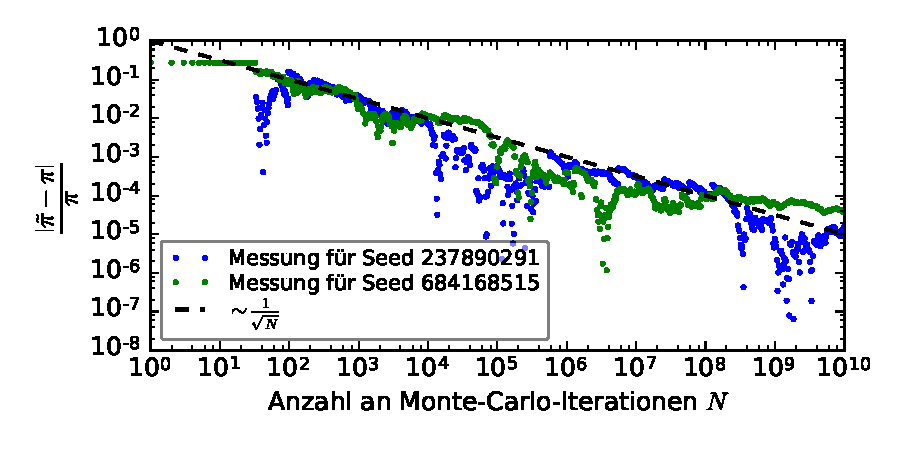
\includegraphics[width=\linewidth]{monte-carlo-pi-error-scaling}
    \end{minipage}
    \caption{Relativer Fehler auf die per Monte-Carlo-Integration berechnete Approximation für Pi für zwei verschiedene PRNG-Seeds.}
    \label{fig:monteerrorfloat}
\end{figure}


%%%%%%%%%%%%%%%%%%%%%%%%%%%%%%%%%%%%%%%%%%%%%%%%%%%%%%%%%%%%%%%%%%%%%%%%%%%%%%%%
\section{Implementation des Kernels}
%%%%%%%%%%%%%%%%%%%%%%%%%%%%%%%%%%%%%%%%%%%%%%%%%%%%%%%%%%%%%%%%%%%%%%%%%%%%%%%%

In \autoref{lst:pikernel} ist die Implementation der Pi-Berechnung zu sehen.
Die Klasse implementiert das Rootbeer-Kernel-Interface, sodass sie von Rootbeer analysiert und auf die GPU portiert werden kann.
Die \lstinline!gpuMethod!-Methode ist jedoch auch normal vom Host aufrufbar.

Die erste Hälfte des Codes ist nur für das Abspeichern von Argumenten über den Konstruktor zuständig, da \lstinline!gpuMethod! keine Argumente nehmen darf, um von Rootbeer erkannt zu werden.

Jeders MonteCarloPiKernel-Objekt sollte mit einem anderen Seed initialisiert werden, bevor gpuMethod aufgerufen wird, sonst rechnen zwei Threads das gleiche und verfälschen damit die Ergebnisse.

Als Pseudozufallszahlengenerator wird ein simpler linearer Kongruenzgenerator genommen. Als Faktor wird 950706376 genommen, vgl. \cite{fishman82,fishman86}

Auf \lstinline!java.util.Random! wurde verzichtet, weil es in ersten Tests zu langsameren GPU-Berechnungen als auf dem Host führte. Es ist zu vermuten und in weiteren Tests zu beweisen, dass Zugriffe auf externe Bibliotheken von Rootbeer nicht in CUDA-Code umgesetzt werden können, sodass die Argumente an den Host gesendet werden, die Funktion auf dem host aufgerufen wird, und die Ergebnisse wieder an die Grafikkarte gesendet werden.

\begin{lstlisting}[language=Java,caption={Implementation der Monte-Carlo-Integration für Pi},label=lst:pikernel]
import org.trifort.rootbeer.runtime.Kernel;
import org.trifort.rootbeer.runtime.RootbeerGpu;

public class MonteCarloPiKernel implements Kernel
{
    private long[] mnHits;      // speichert Ergebnisse pro Kernelthread
    private long   mRandomSeed; // die Zufallssaat für diesen Kernelthread
    private long   mnDiceRolls; // Anzahl an Iterationen die zu tun sind

    public MonteCarloPiKernel
    (
        long[] rnHits     ,
        long   rRandomSeed,
        long   rnDiceRolls
    )
    {
        mnHits           = rnHits;
        mRandomSeed      = rRandomSeed;
        mnDiceRolls      = rnDiceRolls;
    }
    public void gpuMethod()
    {
        final int  randMax   = 0x7FFFFFFF;
        final long randMagic = 950706376;
        int dRandomSeed = Math.abs( (int) mRandomSeed );
        final int dnDiceRolls = (int) mnDiceRolls;
        long nHits = 0;
        for ( long i = 0; i < dnDiceRolls; ++i )
        {
            dRandomSeed = (int)( (randMagic*dRandomSeed) % randMax );
            float x = (float) dRandomSeed / randMax;
            dRandomSeed = (int)( (randMagic*dRandomSeed) % randMax );
            float y = (float) dRandomSeed / randMax;
            if ( x*x + y*y < 1.0 )
                nHits += 1;
        }
        mnHits[ RootbeerGpu.getThreadId() ] = nHits;
    }
}
\end{lstlisting}

Weiterhin wird auch aus Performancegründen \lstinline!mnDiceRolls! in eine lokale Variable zwischengespeichert. Dies führte auch zu einem signifikanten Geschwindigkeitsgewinn, vermutlich weil die zusätzliche Indirektion über die manuellen Speicherverwaltung von Rootbeer vermieden wird. Aus demselben Grund wird auch nicht direkt in \lstinline!mnHits! der Zähler erhöht, sondern eine temporäre lokale Variable genutzt. Letzteres reduzierte im Test eine laufzeit von \SI{2.25}{\seconds} auf \SI{0.5}{\seconds}.\\

Auch sollte man darauf achten, wenn möglich Fließkommazahlen einfacher statt doppelter Genauigkeit zu nutzen, da Grafikkarten häufig mehr Berechnungseinheiten für einfache Genauigkeit besitzen.\\

Abschließend kann man sagen, dass ein erster Rootbeer-Kernel-Prototyp schnell geschrieben ist und teilweise durch Kopieren und Einfügen von normalen Java-Code möglich ist. Aber damit der Kernel auch wirklich schneller auf der Grafikkarte als auf dem Host ist, ist häufig genaues Wissen darüber wie Grafikkarten und auch wie Rootbeer arbeitet nötig.


%%%%%%%%%%%%%%%%%%%%%%%%%%%%%%%%%%%%%%%%%%%%%%%%%%%%%%%%%%%%%%%%%%%%%%%%%%%%%%%%
\section{Rootbeer-Kernelaufruf}
%%%%%%%%%%%%%%%%%%%%%%%%%%%%%%%%%%%%%%%%%%%%%%%%%%%%%%%%%%%%%%%%%%%%%%%%%%%%%%%%

Um einen Rootbeer-Kernel auf einer Grafikkarte auszuführen, muss zuerst ein Rootbeerkontext angelegt werden.
Der Konstruktor des Rootbeerkontexts bereitet die Berechnungen vor, indem es die Rootbeerprogrammbibliotheken aus dem JAR-Archiv in ein temporäres Verzeichnis entpackt. In der originalen Version war dies \lstinline!$HOME/.rootbeer/!.
Dies führt jedoch zu Problemen falls wie auf dem Testsystem, vgl. \autoref{sct:taurus}, das Verzeichnis über alle Knoten gemeinsam verfügbar ist, oder aber auch schon falls Rootbeer thread- oder prozessparallel ausgeführt wird.
Im eigenen Fork \cite{ownrootbeerfork} wird dies mit Commit \lstinline!6196bfd! gelöst, indem die benötigten Programmbibliotheken in ein Unterverzeichnis entpackt wird, welches sich aus Hostname, Prozess-ID, Thread-ID und Nanosekundenzeitstempel zusammensetzt.
Das Rootbeer-Objekt \lstinline!mRootbeerContext! stellt die Methoden \lstinline!getDevices!, \lstinline!createDefaultContext!, \lstinline!getThreadConfig! und \lstinline!run! zur Verfügung.

Die \lstinline!run!-Methode nimmt eine liste von Kernel-Objekten als Argument und für diese auf der Grafikkarte aus. In Multi-GPU-Umgebungen wird die Grafikkarte jedoch autoamtisch gewählt, sodass diese Funktion vermieden werden sollte, stattdessen werden Teile des Quellcodes kopiert und abgeändert, siehe \autoref{lst:runOnDevice}.

Mit \lstinline!getDevices! erhält man eine Liste von \lstinline!GpuDevice!-Objekten die alle Informationen über die jeweilige Grafikkarte enthalten, wie z.B. der maximale Grafikkartenspeicher oder die Taktfrequenz. Außerdem können diese Objekte benutzt werden um Rootbeer-Kernel auf der ausgewählten Grafikkarte in Multi-GPU-Umgebungen auszuführen. In \lstinline!lst:kernelinit! werden die Grafikkarteninformationen benötigt um die Seeds und die Anzahl an Iterationen pro Kernelthread zu berechnen.

Der angelegte Rootbeerfork \cite{ownrootbeerfork} reduziert mit Commit \lstinline!e48b9ae! auf Knoten mit sehr vielen Grafikkarten die Initialisierungszeit von \lstinline!getDevices! um ca. \SI{1}{\seconds} pro verfügbare Grafikkarte, indem es die Aufrufe zu \lstinline!cuCtxCreate! und \lstinline!cuCtxDestroy! für jede Grafikkarte einspart. Der einzige Nachteil ist, dass der freie Speicherplatz auf der Grafikkarte nicht mehr in \lstinline!GpuDevice! verfügbar ist.

Als nächstes werden die Rootbeerkernelobjekte mit jeweiligem Seed initialisiert. Es werden so viele Kernelobjekte erstellt wie die Grafikkarte Threads parallel ausführen kann, um Pipelining voll auszunutzen.
Die GTX 760 z.B. hat 1152 CUDA-Kerne über 6 Shared-Multiprozessoren (SMX), also 192 CUDA-Kerne pro SMX. Jeder SMX kann aber 2048 Threads parallel ausführen, um Latenzen durch Pipelining zu verbergen. In diesem Fall würden also 12288 Kernelobjekte erstellt werden.

Commit \lstinline!9610c99! im eigenen Fork behebt diesbezüglich ein Problem, wo \lstinline!getThreadConfig! nicht optimate Konfigurationen liefert. Und zwar wurden immer so viele Threads genutzt wie ein SMX parallel ausführen konnte. Das heißt je mehr SMX eine Grafikkarte hat, desto mehr Rechenleistung blieb ungenutzt, weil z.B. bei obigen Beispiel nur 2048 Threads anstatt der 12288 Threads gestartet wurden und damit Zugriffslatenzen nicht ausreichend überdeckt werden konnten.

\begin{lstlisting}[language=scala,caption={Initialisierung der Rootbeerkernelobjekte, vgl. auch \lstinline!multiNode/multiGpu/scala/MonteCarloPi.scala! \cite{scaromare}},label=lst:kernelinit]
class MonteCarloPi( iGpuToUse : Array[Int] = null )
{
    private val mRootbeerContext  = new Rootbeer()
    private val mAvailableDevices = mRootbeerContext.getDevices()

    def calc( nDiceRolls : Long, rSeed0 : Long, rSeed1 : Long ) : Double =
    {
        val lnWorkPerKernel = distributor.distribute(
                                  lnWorkPerGpu(iGpu),
                                  lnKernelsPerGpu(iGpu)
                              )
        val tasks = lnWorkPerKernel.zipWithIndex.map( x => {
            ...
            new MonteCarloPiKernel(
                lnHits(iGpu)      ,
                kernelSeed        ,
                nWorkPerKernel      /* iterations to do */
            )
        } )
        runState = runOnDevice( mAvailableDevices.get( iGpuToUse ), tasks )
        ...
        runState.take()
    }
}
\end{lstlisting}


Die Funktion \lstinline!runOnDevice!, siehe \autoref{lst:kernelcall}, führt eine Liste aus Kernelobjekten auf der ausgewählten Grafikkarte aus.
Dafür wird auf dem ausgewählten \lstinline!GpuDevice! ein Beschleunigerkontext, also z.B. ein CUDA-Kontext, angelegt. Das Argument an \lstinline!createContext! gibt den voraussichtlich benötigten Grafikkartenspeicher an. Für Rootbeerkernel die dynamisch Speicher alloziieren, z.B. durch einen \lstinline!new!-Operator, ist diese Angabe Pflicht. Leider funktioniert die automatische Speicherberechnung auch von statischen Kernels nicht, sodass man in jedem Fall eine Angabe machen muss. Da man jedoch tiefe Einblicke in die Funktionweise von Rootbeer benötigt, um das abschätzen zu können, sollte so viel Speicher wie möglich als Reserve angefordert werden.

Als nächstes werden die Anzahl für die aus CUDA bekannten Blöcken und Threads festgelegt, die der Kernel umfassen soll. Diese wird berechnet aus der Anzahl an übergebenen Kernelobjekten.

Mit \lstinline!buildState! werden Thread-Konfiguration zwischengespeichert, benötigte Serialisierungsspeicher auf Grafikkarte und Host angelegt und die CUDA-Binärdateien der vorkompilierten Kernel geladen und an den CUDA-Kontext gesendet.

Letztendlich werden mit \lstinline!runAsync! alle benötigten Daten vom Host an die Grafikkarte übertragen und der Kernel in einem eigenen Thread gestartet. Zurückgegeben wird ein \lstinline!GpuFuture!-Objekt mit einer \lstinline!take!-Methode, mit der auf die Vollendung des Threads gewartet werden kann, siehe \autoref{lst:kernelinit}. Dies ermöglicht das Nutzen mehrere Grafikkarten parallel aus einem Thread oder Prozess heraus, ohne dass sich der Rootbeernutzer selbst um Multithreading kümmern muss.

\begin{lstlisting}[language=scala,caption={Ausführen der Rootbeerkernels auf einer ausgewählten Grafikkarte, vgl. auch \lstinline!multiNode/multiGpu/scala/MonteCarloPi.scala! \cite{scaromare}},label=lst:kernelcall]
    def runOnDevice(
        device : GpuDevice,
        work   : List[Kernel]
    ) : Tuple2[ Context, GpuFuture ] =
    {
        val context = device.createContext( 128*1024*1024 )
        val threadsPerBlock = 256;
        val thread_config = new ThreadConfig(
            threadsPerBlock, /* threadCountX */
            1,               /* threadCountY */
            1,               /* threadCountZ */
            ( work.size + threadsPerBlock - 1 ) / threadsPerBlock, /* blockCountX */
            1,               /* blockCountY */
            work.size        /* numThreads */
        );
        context.setThreadConfig( thread_config )
        context.setKernel( work.get(0) )
        context.setUsingHandles( true )
        context.buildState()
        val runWaitEvent = context.runAsync( work )
        return ( context, runWaitEvent )
    }
\end{lstlisting}


%%%%%%%%%%%%%%%%%%%%%%%%%%%%%%%%%%%%%%%%%%%%%%%%%%%%%%%%%%%%%%%%%%%%%%%%%%%%%%%%
\section{Kombination von Rootbeer mit Spark}
%%%%%%%%%%%%%%%%%%%%%%%%%%%%%%%%%%%%%%%%%%%%%%%%%%%%%%%%%%%%%%%%%%%%%%%%%%%%%%%%

Die Idee ist einfach, man nutzt die Map-Funktion eines RDD, um z.B. eine Liste an Seeds abzubilden auf die Ergebnisse der Rootbeerkernel, indem man die Logik aus \autoref{lst:kernelinit} kopiert.
Dabei stellen sich jedoch mehrere Probleme.

Wenn eine Partition auf eine Grafikkarte abgebildet wird und Workerknoten mehrere Grafikkarten besitzen, dann muss Rootbeer thread-safe sein. Dies wurde erst mit Commit \lstinline!aa3a0bc! und dem schon erwähnten Extraktionspfadproblem in Commit \lstinline!6196bfd! im Fork \cite{ownrootbeerfork} gelöst. Rootbeer war nicht thread-safe, da es an vielen Stellen nicht benötigte Singletons und statische Variablen verwendet. Der Compiler selbst ist immer noch nicht thread-safe, nur die Laufzeitklassen.

Bei Knoten mit mehreren Grafikkarten muss darauf geachtet werden, dass nicht zwei Partitionen derselben Grafikkarte zugeteilt werden.
Als Voraussetzung ist dafür ein Partitionierer von Nöten, der die Partitionen exakt verteilt.
Nutzt man den Standardpartitionierer, so kam es in Tests häufig vor, dass bei gleich vielen Kernen wie Elementen jeder Knoten bis auf zwei so viele Elemente zugewiesen bekommt, wie er Knoten hat. Ein Knoten jedoch kriegt ein Element weniger und ein anderer eins mehr. Um dieses Problem zu beheben wird ein benutzerdefinierter Partitionier benutzt.
\begin{lstlisting}[language=Scala,caption={Exakter Partitionierer},label={lst:exactpart}]
class ExactPartitioner[V]( partitions: Int, elements: Int) extends Partitioner {
    def numPartitions() : Int = partitions
    def getPartition(key: Any): Int = key.asInstanceOf[Int] % partitions
}
\end{lstlisting}
Mit Hilfe dieser Klasse kann nun Informationen über den RDD bzw. die Sparkinstanz gesammelt werden.
\begin{lstlisting}[language=Scala,caption={Ausschnitt aus \lstinline!getClusterGpuConfiguration!, vgl. \lstinline!multiNode/multiGpu/scala/TestMonteCarloPi.scala!},label=lst:clusterconfig}
val configuration = sc.
    parallelize( (0 until nPartitions).zipWithIndex ).
    partitionBy( new ExactPartitioner( nPartitions, nPartitions ) ).
    map( x => {
        val devices = (new Rootbeer()).getDevices
        val totalPeakFlops = devices.toList.map( x => {
            x.getMultiProcessorCount.toDouble *
            x.getMaxThreadsPerMultiprocessor.toDouble *
            x.getClockRateHz.toDouble
        } ).sum
        /* return */
        ( /* key */ InetAddress.getLocalHost.getHostName,
          /* val */ ( devices.size, totalPeakFlops ) )
    } ).
    cache /* ! */
\end{lstlisting}
In \autoref{lst:clusterconfig} bezeichnet \lstinline!sc! den Sparkkontext. Die \lstinline!partitionBy!-Methode ermöglicht es den RDD mit dem obig beschriebenen benutzerdefinierten Partitionierer


%%%%%%%%%%%%%%%%%%%%%%%%%%%%%%%%%%%%%%%%%%%%%%%%%%%%%%%%%%%%%%%%%%%%%%%%%%%%%%%%
\section{Kompilierung}
%%%%%%%%%%%%%%%%%%%%%%%%%%%%%%%%%%%%%%%%%%%%%%%%%%%%%%%%%%%%%%%%%%%%%%%%%%%%%%%%


\begin{figure}[H]
    \centering
    \begin{minipage}{\linewidth}
        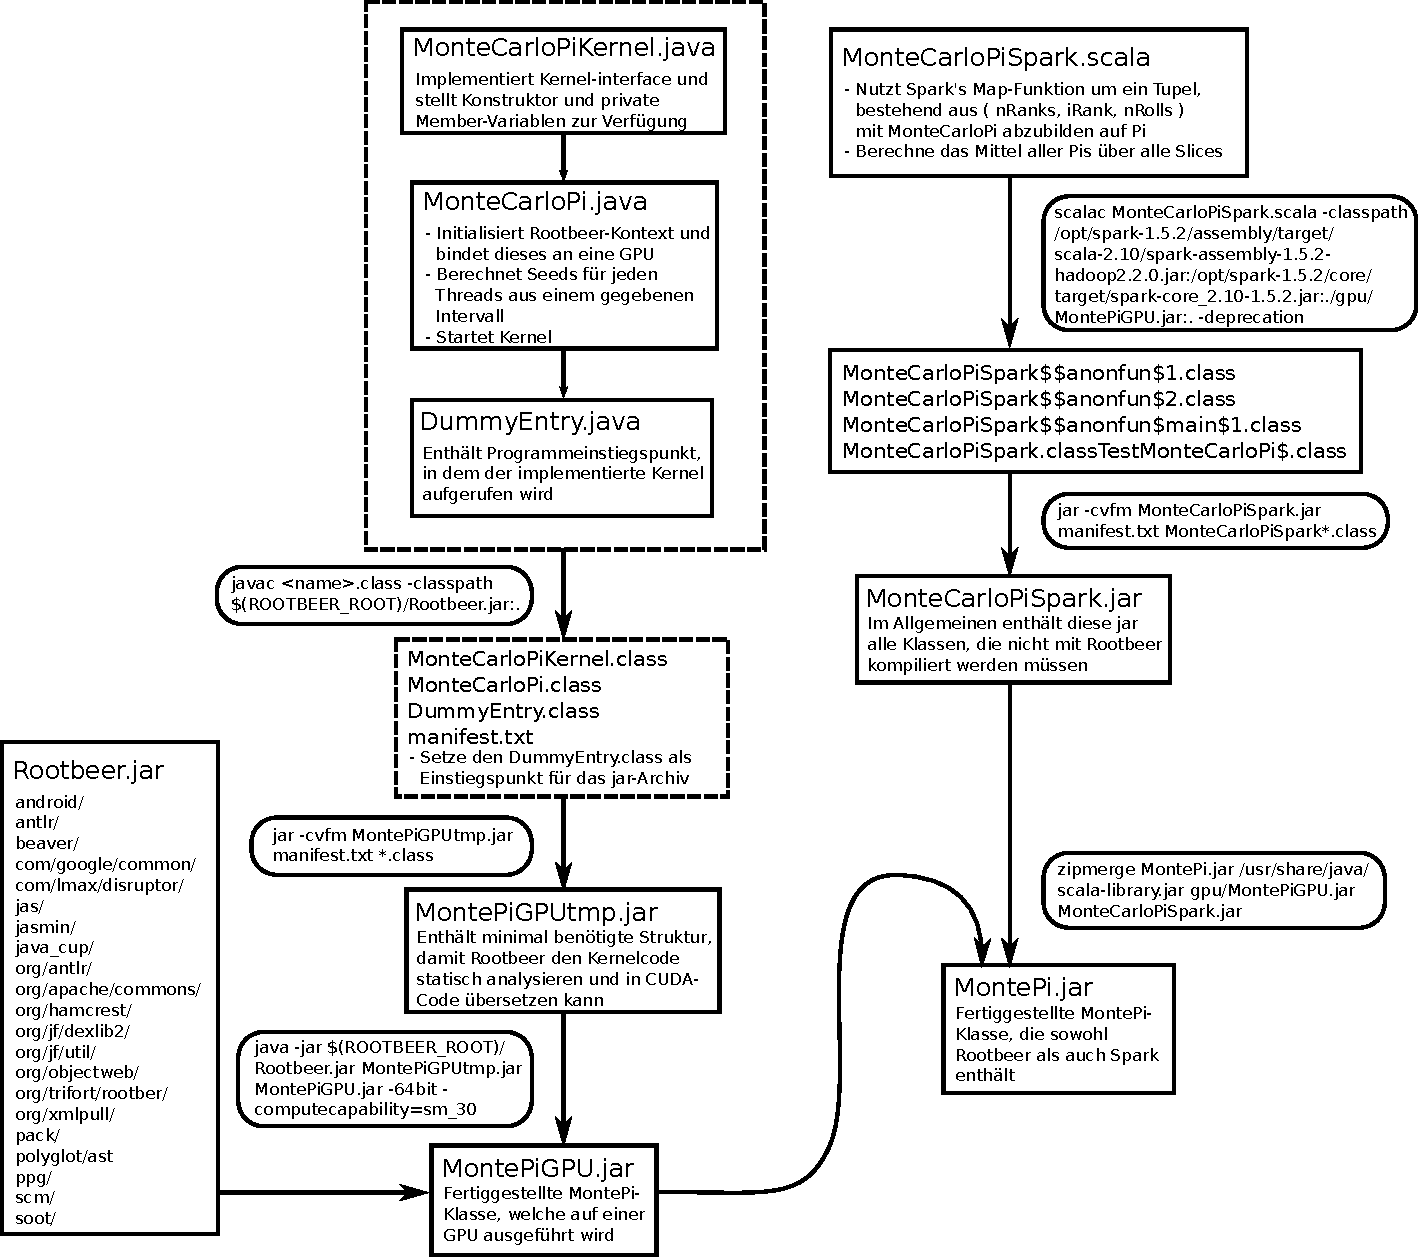
\includegraphics[width=\linewidth]{compile-structure-deu.pdf}
    \end{minipage}
    \caption{Kompilationsschema mit Kommadozeilenbefehlen und Zwischenstati.}
    \label{fig:compilation}
\end{figure}

!!! Problem: Hab mehrere Fehler gefunden deren Kenntnis möglicherweise eine Vereinfachung des Schemas bedeutet. Da bin ich noch am rumspielen, daher ist das halbfertig.

\section{Probleme}
Implementierung:
    Was ist bei GPUs zu beachten ( Seeds, 64-Bit )
    Was ist bei Rootbeer zu beachten?
      - private Variablen werden wirklich immer per memcpy hin und her transportiert.
      - muss nicht auf ungerade Kernel-Zahl achten, werden automatisch aussortiert
